\documentclass[a4paper]{article}

%% Language and font encodings
\usepackage[english]{babel}
\usepackage[utf8x]{inputenc}
\usepackage[T1]{fontenc}
\usepackage{subfig}
\usepackage{multirow}
\usepackage{array}
\usepackage[noend]{algpseudocode}
\usepackage{algorithm}

%% Sets page size and margins
\usepackage[a4paper,top=3cm,bottom=2cm,left=3cm,right=3cm,marginparwidth=1.75cm]{geometry}

%% Useful packages
\usepackage{amsmath}
\usepackage{graphicx}
\usepackage[colorinlistoftodos]{todonotes}
\usepackage[colorlinks=true, allcolors=blue]{hyperref}

\title{Calculating Set Difference Among Sets Stored in Bloom Filters}
\author{Neha Sengupta \and Pratham Shah \and Shubham Jain}
\begin{document}
\maketitle

\section{Introduction}
Bloom Filters {\cite{2}} are data structures that can efficiently answer set-membership queries.  Swamidass \& Baldi (2007) {\cite{3}} demonstrated how size of union and intersection of two sets represented using Bloom Filters can be estimated. However, a very fundamental problem of calculating set difference among two sets stored as Bloom Filters remains solved. In this paper, we give a method to estimate elements in the set difference among two sets represented as Bloom Filters. \newline
\textit{Problem Statement}. If we are given two sets $S1$ and $S2$ from a namespace $U$ stored in Bloom Filters $B1$ and $B2$ respectively, then we try to estimate elements that are in $S1$ but not in $S2$. \newline
$Solution Overview.$ We exploit Bloom Sample Tree {\cite{1}} to represent the entire namespace. We go down the tree estimating number of common elements between nodes of the tree and $S1$ and $S2$. If no common element with $S1$ is found, search along that path is pruned, if no common element with $S2$ is found, the node is added into the result and if there are common elements with both sets are found, we move a level down on the path.

\section{Algorithm}
The following algorithm is used to estimate elements in the set difference among two sets $S$ and $C$ represented as Bloom Filters using Bloom Sample Tree $B$ which represents namespace where $B_{ij}$ represents $j^{th}$ node of $i^{th}$ level.

\begin{algorithm}
\caption{$Set\_diff (B_{ij}, S, C)$}
\begin{algorithmic}[1]
\Procedure{Set\_diff}{$B_{ij}, S, C$}
 \If{$isLeaf(B_{ij})$}
    \State \textbf{return} all elements of $B_{ij}$ that are in $S$ and not in $C$
  \ElsIf{$B_{ij} \cap S = \phi$}
    \State  \textbf{return} $\phi$
     \ElsIf{$B_{ij} \cap C = \phi$}
    \State  \textbf{return} $S$
    \Else 
    \State
    \textbf{return} $Set\_diff (B_{i+1,2j}, S, C) \cup Set\_diff (B_{i+1,2j+1}, S, C)$
  \EndIf
\EndProcedure
\end{algorithmic}
\end{algorithm}



\begin{algorithm}
\caption{$Set\_difference (B_{ij}, S, C)$}
\begin{algorithmic}[1]
\Procedure{Set\_difference}{$B_{ij}, S, C$}
 \State 
 \textbf{return} $Set\_diff (B_{0,0}, S, C)$
\EndProcedure
\end{algorithmic}
\end{algorithm}







\section{Experimental Evaluation}
In this section, we describe the experiments we did with different approaches using static namespace. We compared running time of different approaches to generating a single sample required number of times.

\subsection{Setup}
We used a static synthetic namespace to compare running time of the different  approaches. We varied our namespace from $10^5$ to $10^7$. We also varied number of samples to be generated from $1000$ to $10000$.In the combined approach, we have used 256 threads for the below experiments. \newline
\textbf{Query Sets} In the experiments we performed, we generated query sets uniformly at random from the the entire namespace.
\newline
\textbf{Algorithms} We compared running time of approaches $2$ and $3$ and compare it to running time of generating a single sample required number of times.
\newline
\textbf{Metrics} We report the running time of algorithms by running them multiple times and taking average over the running times.


\section{Results}
Figure 1 shows the average time taken to sample multiple elements from a set using a Bloom Sample Tree using different approaches. The experiment demonstrate that creating multiple threads in advance and then using each to handle multiple nodes is the best strategy of the proposed ones.
\begin{figure}[h!] 
\centering
\begin{tabular}{cccc}
\subfloat[$m=10^4$, $n=10^4$, $M=10^5$]{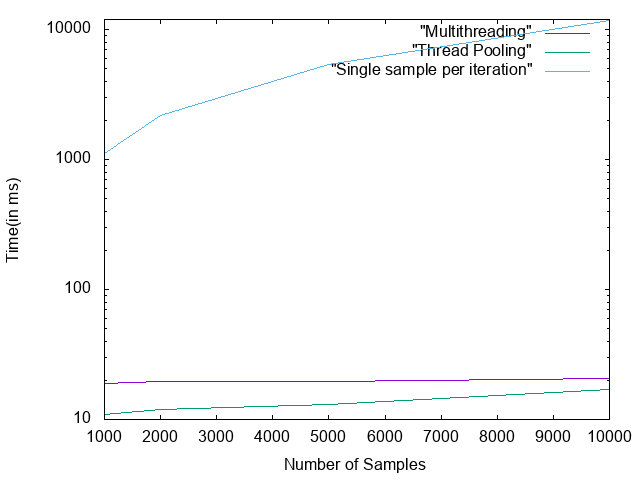
\includegraphics[width=0.5\textwidth]{plot5.png}} 
\subfloat[$m=10^5$, $n=10^4$, $M=10^6$]{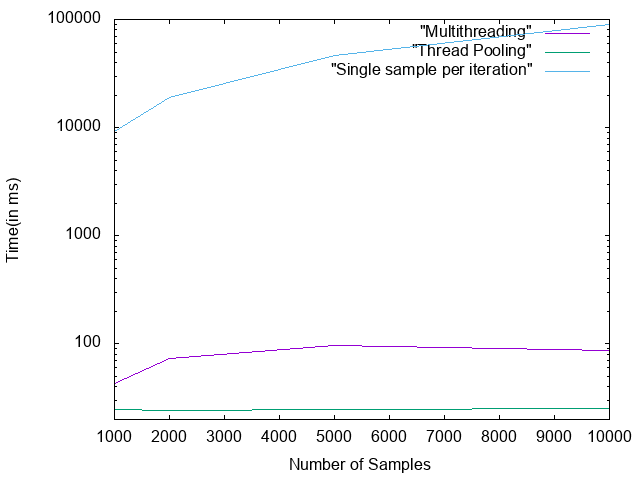
\includegraphics[width=0.5\textwidth]{plot6.png}}\\
\subfloat[$m=10^6$, $n=10^4$, $M=10^7$]
{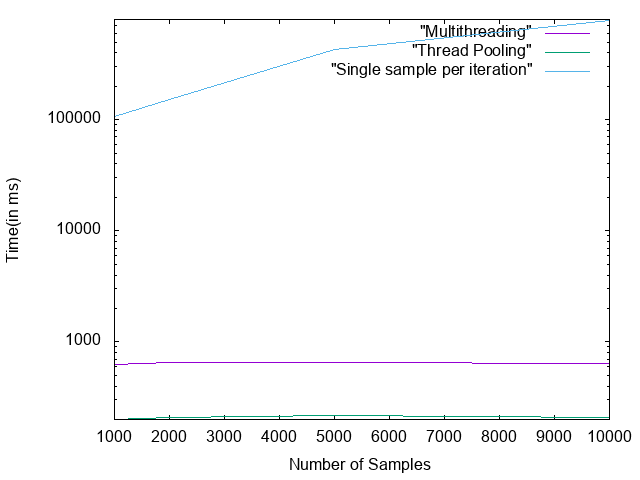
\includegraphics[width=0.5\textwidth]{plot7.png}}
\subfloat[$m=10^6$, $n=10^4$, $M=10^8$]
{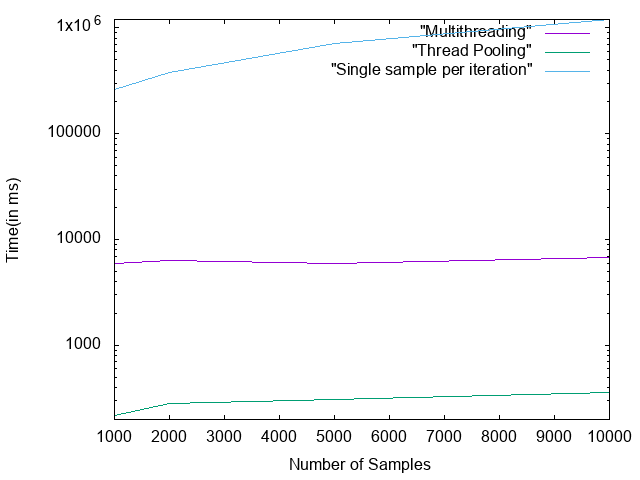
\includegraphics[width=0.5\textwidth]{plot8.png}}
\end{tabular}

\caption{\label{fig:plot}Time taken for different approaches}
\end{figure}

\section{Conclusions}
In this paper, we described different methods of sampling multiple elements using a Bloom Sample Tree and compared the time taken by them in different settings. Our experiments demonstrated that the most suitable approach out of the approaches mentioned is to create multiple threads prior to sampling, and then using each of the threads to handle multiple nodes in the Bloom Sample Tree.
\bibliographystyle{alpha}
\bibliography{sample}

\end{document}